\chapter{Wordpress: applicazione pratica dello strumento realizzato}

Al fine di verificare iil funzionamento e l'effettiva efficacia del software proposto e delle strategie analizzate, si è scelto di eseguire alcune prove pratiche di utilizzo in situazioni reali. 

La prima decisione che è stata presa in questo senso ha riguardato l'applicazione web da esaminare. La scelta finale è ricaduta su Wordpress, per i motivi che verranno ora elencati.

Wordpress è l'applicazione web per la pubblicazione la gestione di blog più diffusa al momento, ed è usato come piattaforma di pubblicazione dei contenuti da decine di milioni di siti web \footnote{\url{http://en.wordpress.com/stats}}. Vista l'enorme diffusione, rappresenta un caso interessante e significativo.

Il progetto è open source sviluppato in PHP, pertanto è possibile accedere al codice sorgente per analizzarne se necessario il funzionamento \footnote{\url{http://core.svn.wordpress.org/trunk}}. Nel codice repository dei test accessibile pubblicamente \footnote{\url{http://svn.automattic.com/wordpress-tests}} è presente solamente una suite di unit test, pertanto realizzare una serie di test di più alto livello non si è rivelato un esercizio unicamente fine a sé stesso.

Si possiede poi già esperienza sia nell'utilizzo che nell'estensione di questa piattaforma, pertanto è stato possibile individuare facilmente gli scenari di interesse per i test di accettazione, cercando di evidenziare gli scenari di maggiore interesse per valutare il comportamento dello strumento di testing realizzato. 

In aggiunta, la parte di front-end della piattaforma in esame, ossia il pannello di amministrazione, presenta un codice HTML di concezione moderna, ben strutturato ed utilizzato prevalentemente in maniera semantica. Grazie a ciò lo strumento di testing si deve confrontare con un'applicazione web che presenta un sufficiente livello di qualità nella realizzazione dell'interfaccia utente, adatto a soddisfare almeno in parte i requisiti consigliati per il suo impiego.

Infine, l'interfaccia non è particolarmente complessa e non viene fatto un uso intensivo della tecnologia Ajax, utilizzata più che altro per migliorare l'esperienza dell'utente in alcune funzionalità marginali. Anche l'organizzazione dei contenuti e le strutture nel DOM del pannello di amministrazione sono piuttosto tipici, pertanto il back-end di Wordpress può essere preso come un campione rappresentativo di molte piattaforme analoghe.

Lo scenario di test analizzato prevede alcune operazioni comuni all'interno del sistema Wordpress, come l'accesso dell'amministratore dalla pagina di login e l'inserimento di un nuovo articolo del blog. La sequenza delle operazioni è stata registrata e poi riprodotta sulla versione 2.8 di Wordpress, installata in locale. 

In un secondo momento, lo stesso test definito in precedenza è stato riprodotto sulla versione 3.1, che presenta alcune differenze nel layout grafico, nella distribuzione dei contenuti e nella struttura dell'HTML, rimanendo però analoga sia per le funzionalità offerte sia per il modo in cui esse sono raggiungibili dall'utente. 

In questo modo è stato possibile fare una prima valutazione pratica circa la resistenza dei test registrati ai cambiamenti nel DOM delle pagine, considerando un caso reale di evoluzione nell'interfaccia e non semplicemente una serie di modifiche studiate ad hoc.

\section{Descrizione del primo esperimento}

\subsection{Preparazione dello strumento e definizione del punto di partenza per il test}

Una volta avviato il programma, si attiva la modalità di registrazione premendo l'apposito pulsante nella barra degli strumenti principale, si digita l'indirizzo stabilito come punto di partenza per il test e si preme il pulsante "Visit". Poiché si è in modalità di registrazione, viene creata la prima azione nella lista a destra della finestra. Questa azione corrisponde alla navigazione dell'utente ad un indirizzo specificato ed essendo la prima che è stata definita farà in modo che il simulatore si porti sempre sulla pagina iniziale prima di effettuare le altre azioni.

\begin{figure}[htbp]
\begin{center}
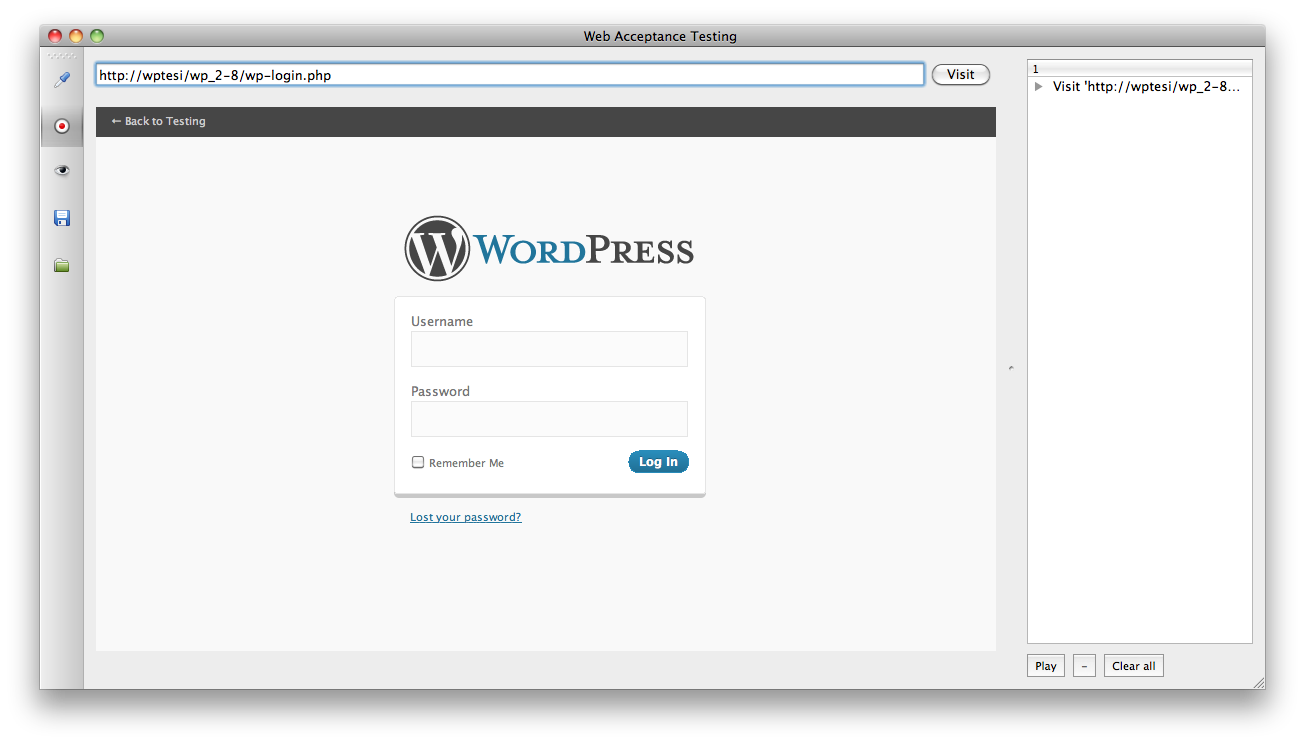
\includegraphics[width=\textwidth]{images/wp_tour/1_login.png}
\end{center}
\end{figure}
 

\subsection{Pagina di login}

Sempre con la modalità di registrazione attivata, si inseriscono il nome utente e la password negli appositi campi. Quando una casella di testo perde il focus ed il suo contenuto non è nullo, viene aggiunta l'azione "Fill input", che rappresenta l'inserimento di una serie di caratteri da parte dell'utente nella casella di testo correntemente attiva. 

Espandendo la riga dell'azione di tipo "Fill input" appena creata, si può osservare che sono state registrate automaticamente anche due informazioni essenziali per riprodurre in seguito l'azione, ossia il selettore ed il valore immesso nel campo. Scendendo nel dettaglio, l'evento Javascript \verb|blur| viene intercettato dal codice presente nel file \verb|logger.js|. Tramite jQuery viene reperito il valore presente nel campo di testo e viene cercato un tag di tipo \verb|label| associato al campo tramite l'attributo \verb|for|, oppure che contenga al suo interno il campo. Se l'etichetta viene trovata, se ne ottiene il testo contenuto.

Inoltre, viene richiamata la funzione che costruisce il selettore secondo l'algoritmo esposto in precedenza, passando come argomento il riferimento al nodo del DOM corrente, ossia il campo di testo.

A questo punto viene richiamato nello script l'apposito metodo dell'oggetto Python di classe \verb|Logger|, reso disponibile nel contesto della pagina sotto forma di oggetto Javascript, passando come parametri il selettore, il valore del campo, il ed il contenuto della label, se presente. Quest'ultimo viene mostrato all'utente nella lista delle azioni in modo che sia chiaro quale campo è stato compilato, rendendo più leggibile il test che si sta registrando.

\begin{figure}[htbp]
\begin{center}
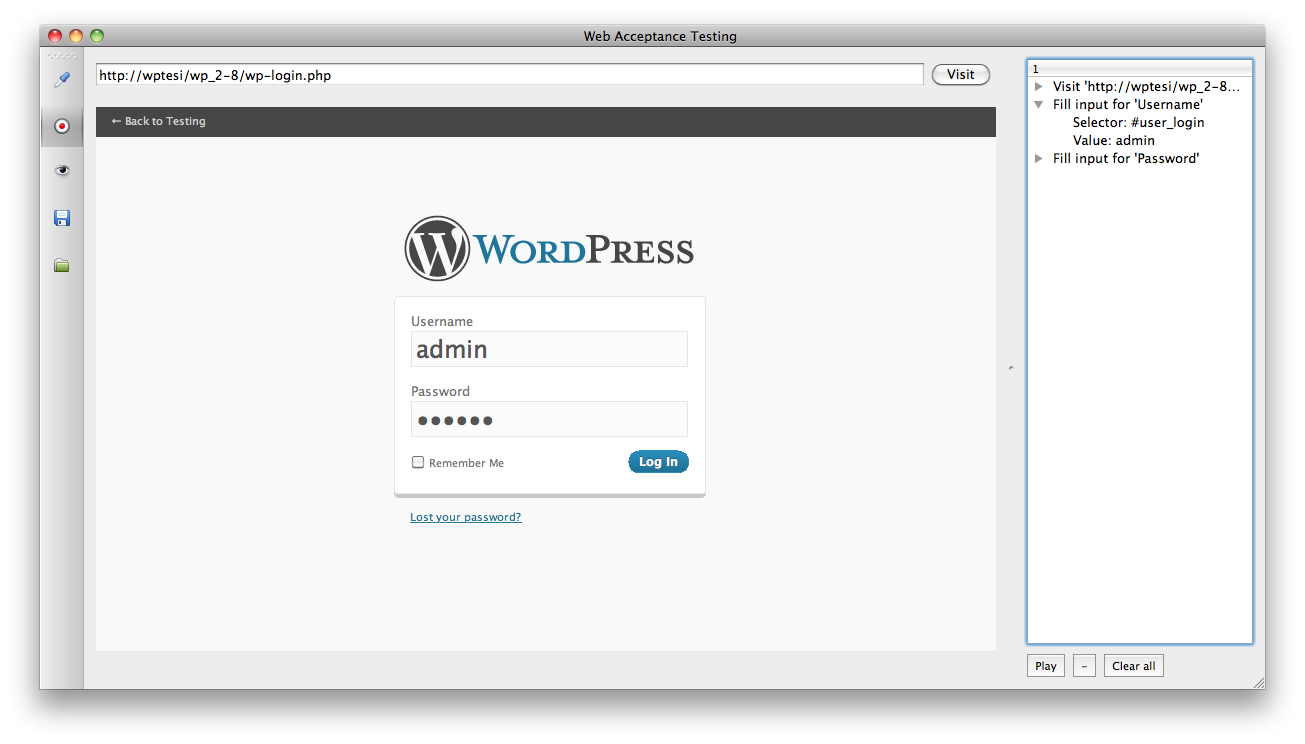
\includegraphics[width=\textwidth]{images/wp_tour/2_fill_login.png}
\end{center}
\end{figure}

Premendo poi il pulsante "Login" viene registrata l'azione corrispondente, in maniera analoga a quanto appena descritto. Fino a che il caricamento della pagina successiva non è completato, viene mostrato un messaggio che avvisa di attendere e viene inibita la registrazione di nuove azioni, per evitare possibili inconsistenze dovute alla situazione non stabile della pagina. Inoltre viene aggiornato il contenuto della barra dell'indirizzo con l'url della pagina corrente.

\subsection{Dashboard}

Una volta terminato il login, si procede a definire la prima asserzione, che permette di assicurarsi che il login sia effettivamente andato a buon fine e che ci si trovi nella pagina della dashboard. 

Per fare ciò, dopo aver cliccato sul pulsante nella barra degli strumenti per aggiungere una nuova asserzione, viene aperta una finestra di dialogo attraverso la quale inserire le informazioni per la nuova asserzione. Si procede selezionando il tipo di asserzione da aggiungere, scegliendo tra quelle disponibili. Per il tipo "Element contains" viene controllato in fase di riproduzione che l'elemento specificato sia presente nella pagina e nel testo contenuto sia presente la stringa di testo specificata nell'apposito campo.

Il selettore all'elemento che sarà oggetto della verifica può essere inserito manualmente, oppure può essere generato automaticamente dall'algoritmo. Per seguire questa seconda opzione, è necessario cliccare sul pulsante "Pick". La finestra di dialogo sarà così temporaneamente nascosta e sulla pagina verrà attivata la modalità di selezione. 

In questa modalità, viene disegnato tramite Javascript un bordo attorno all'elemento sottostante al puntatore del mouse, cosicché l'utente possa scegliere l'elemento che deve essere oggetto dell'asserzione cliccando sull'elemento evidenziato.

Per realizzare questa funzionalità, si è rivelato necessario posizionare quattro nodi di tipo \verb|div| intorno all'elemento target dell'evento \verb|mouseover|. Questi elementi fittizi vengono posizionato in maniera assoluta e sovrapposti al contenuto della pagina tramite la regola CSS \verb|z-index|. Ognuno di essi rappresenta una delle quattro regioni attorno al rettangolo che individua virtualmente l'elemento sotto il puntatore del mouse, e per ciascuno viene impostato tramite CSS un bordo rosso per il lato che combacia con l'elemento. Questa soluzione più complicata si è resa necessaria per evitare possibili interferenze con il layout della pagina dovute al modo in cui opera il box model, nel caso in cui le larghezze degli elementi siano definite in maniera precisa.

Se si fosse semplicemente assegnato un bordo all'elemento da evidenziare si sarebbero infatti alterate le dimensioni dell'elemento, poiché lo spessore del bordo viene conteggiato sia nel calcolo dell'altezza che in quello della larghezza dell'elemento. Questo può provocare uno spostamento indesiderato nel layout della pagina, qualora l'allineamento degli elementi dipenda dalle esatte dimensioni degli stessi.

Una volta che viene effettuato il click sul nodo evidenziato, quest'ultimo viene passato come parametro di ingresso all'algoritmo di generazione dei selettori. Dal contesto Javascript il selettore ed il testo contenuto nell'elemento vengono resi disponibili alla parte in Python tramite l'oggetto condiviso di classe \verb|Logger|. Quando esso emette il segnale PyQt \verb|pathPicked|, l'applicazione può mostrare nuovamente la finestra di dialogo, con il campo per specificare il selettore impostato al valore generato via Javascript.

Una volta applicate le impostazioni per la nuova asserzione, viene creata la relativa riga nella lista delle azioni registrate. Durante la fase di riproduzione, l'asserzione verrà eseguita quando il simulatore raggiungerà lo step corrispondente, secondo l'ordine mostrato.

Per questa asserzione, il selettore restituito risulta essere \verb|#wpbody-content h2|. La struttura del DOM in cui si trova l'elemento è quella mostrata in figura ~\ref{fig:dashboardH2DOM}, ricavata tramite l'estensione Firebug. Come si può osservare, il selettore generato non tiene conto del nodo \verb|div.wrap|, poiché esiste un solo tag \verb|h2| all'interno del sottoalbero che ha come radice il nodo \verb|div#wpbody-content|. 

\begin{figure}[htbp]
\begin{center}
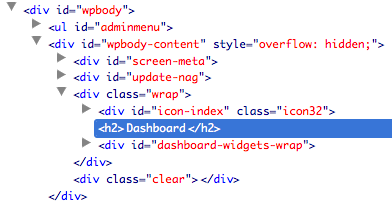
\includegraphics[width=\textwidth]{images/wp_tour/7_dashboard_h2_firebug.png}
\caption{Porzione dell'albero del DOM per il titolo "Dashboard"}
\label{fig:dashboardH2DOM}
\end{center}
\end{figure}

\subsection{Pagina per la pubblicazione di un nuovo articolo}

\subsubsection{Click nel menù principale}

Per raggiungere la pagina di inserimento di un nuovo articolo, si clicca sulla voce nel menù principale a sinistra. Viene registrata l'azione corrispondente e il selettore ottimizzato restituito per il collegamento cliccato è \verb|#menu-posts a:icontains(add+new)|. La reale struttura del DOM è mostrata in figura ~\ref{fig:addNewDOM}: in questo caso i nodi intermedi tra il collegamento ipertestuale ed il nodo \verb|li#menu-posts| sono stati ignorati dall'algoritmo e non compaiono nel selettore finale. Siccome poi è stata utilizzata una lista di tipo non ordinato, nel selettore non è presente un'indicazione sulla posizione della voce contenente il link cliccato. E' pertanto possibile aggiungere nuove voci al menù, oppure modificare l'ordinamento delle voci o il tipo di tag utilizzati, senza dover modificare il test in un secondo momento. Una modifica che invece potrebbe rendere necessaria la ridefinizione di questo passaggio nel test consiste nell'aggiungere una nuova voce nel menù che contenga la stringa "add new" in posizione precedente rispetto al nodo di riferimento.

Siccome nel codice HTML è stato assegnato un attributo \verb|id| alla voce del menù che contiene a sua volta il sottomenù con i collegamenti per le azioni riguardanti gli articoli, il test verifica anche implicitamente che il collegamento "Add new" si trovi nella corretta sezione del menù. La sezione riguardante le azioni sugli articoli è infatti identificata dal sottoalbero identificato dall'algoritmo tramite l'attributo \verb|id| definito sulla voce della lista.

\begin{figure}[htbp]
\begin{center}
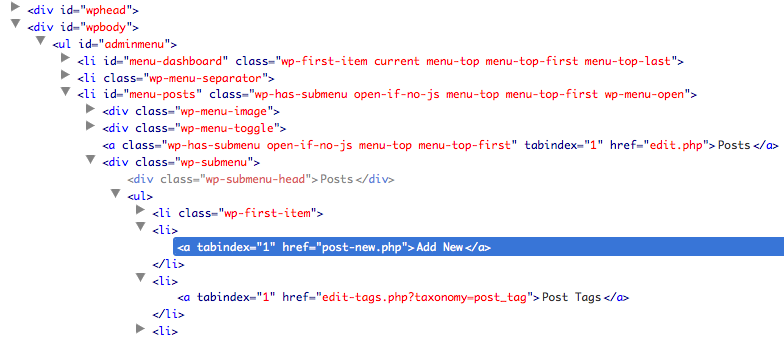
\includegraphics[width=\textwidth]{images/wp_tour/8_add_new_firebug.png}
\caption{Porzione dell'albero DOM per il menù principale}
\label{fig:addNewDOM}
\end{center}
\end{figure}

A questo punto viene inserito il testo del titolo per il nuovo articolo. Il tag HTML del campo possiede un attributo di tipo \verb|id|, quindi il selettore generato risulta essere semplicemente \verb|#title|. Nel caso in cui non fosse stato definito questo attributo, l'algoritmo avrebbe utilizzato l'attributo \verb|name| per identificarlo.

\subsubsection{Creazione ed assegnamento di una nuova categoria via Ajax}

Il passo successivo nel test prevede l'assegnamento dell'articolo ad una nuova categoria. Per facilitare questa operazione, tramite l'interfaccia l'utente può creare direttamente una nuova categoria prima di selezionarla, senza dover lasciare la pagina corrente. La nuova categoria verrà infatti salvata nel database tramite una richiesta asincrona.

Questa operazione ha fatto emergere poi un altro interessante aspetto, che ha richiesto un ripensamento della strategia con cui vengono intercettati gli eventi tramite Javascript.

Il campo per inserire il titolo della nuova categoria e il bottone di conferma sono inizialmente nascosti, e vengono mostrati solamente dopo il click sul link "Add new category". Durante i primi esperimenti, l'evento di click su questo link non veniva però intercettato dal codice Javascript utilizzato per la registrazione.

Dopo aver analizzato la porzione del codice di Javascript usato in Wordpress per questa operazione, riportato nel listato ~\ref{code:wpReturnFalse} ci si è accorti che il problema risiede nel fatto che la funzione ritorna il valore \verb|false|.
Questo valore viene restituito poiché si desidera che il browser non esegua l'operazione tipica che accade al click su di un link, ossia la visita dell'indirizzo (o del frammento) specificato nell'attributo \verb|href|. Come effetto collaterale però viene annullata la propagazione dell'evento nel DOM, che non raggiungerà mai il nodo \verb|body|, sul quale sono definiti gli event handler tramite il metodo jQuery \verb|.live|, che intercettato gli eventi per la registrazione.

In realtà il problema non si sarebbe posto se fossero stati usati nel codice di Wordpress i metodi Javascript adatti. Gli oggetti di tipo \verb|event| possiedono infatti alcuni metodi apposta per avere un maggiore controllo in questa situazione: sarebbe stato più adeguato utilizzare il metodo \verb|event.preventDefault|, che impedisce proprio al browser di eseguire l'azione standard ma non blocca la propagazione dell'evento.

\lstinputlisting[float=h, language=Javascript, caption={Codice Javascript usato in Wordpress per mostrare i campi nascosti}, label=code:wpReturnFalse]{code/wp/return_false.js}

La risoluzione di questo problema ha infine portato ad implementare una strategia migliore per la registrazione degli eventi, che evita il verificarsi di situazioni analoghe.

Essa consiste nello sfruttare la prima fase di propagazione degli eventi, definita dalla specifica Document Object Model Level 3 [http://www.w3.org/TR/DOM-Level-3-Events/]. Come descritto in precedenza, in questa fase gli eventi vengono propagati in maniera top-down nell'albero, ed è possibile usare il parametro \verb|useCapture| del metodo \verb|addEventListener| per associare una funzione di callback che intercetta l'evento esclusivamente durante questa fase.

Così facendo l'evento viene comunque registrato, anche se il codice Javascript presente nell'applicazione sotto esame ne annulla la propagazione per qualche motivo. Di fatto viene ridotta notevolmente la possibilità di interferenze tra il codice iniettato e quello definito dall'applicazione. Nel listato ~\ref{code:eventCapturing} viene mostrato un esempio di questa soluzione.

\lstinputlisting[float=h, language=Javascript, caption={Definizione degli event handler per la fase di capturing}, label=code:eventCapturing]{code/wp/capture.js}

\subsubsection{Verifica dell'inserimento e del filtro di ricerca}

Una volta assegnata la categoria e il titolo dell'articolo, si preme sul pulsante "Publish", viene registrata l'azione corrispondente e l'articolo viene salvato nel database dell'applicazione. 

A questo punto si vuole verificare che l'utente si ritrovi sulla pagina di modifica del post appena pubblicato e che venga mostrato un messaggio di conferma. Tramite la finestra di dialogo si crea una nuova asserzione e si seleziona il messaggio con sfondo giallo, per il quale viene restituito il selettore \verb|#message|. Si comunica anche di voler controllare che questo elemento contenga la stringa "post published".

Si verifica poi che il campo di testo per il titolo dell'articolo contenga il valore che si era immesso nel passaggio precedente.

Successivamente, si clicca nella voce del menù principale che porta all'elenco degli articoli salvati. Da questa pagina si seleziona dal filtro di ricerca la voce corrispondente al nome della nuova categoria creata, alla quale è stato assegnato l'articolo appena pubblicato. L'azione viene registrata grazie all'evento \verb|change| che si verifica quando l'utente modifica la voce selezionata in un tag di tipo \verb|select|. 

Per effettuare la ricerca si registra l'azione di click sul pulsante "Filter". Nella schermata ci si aspetta di trovare un solo articolo nella categoria appena creata, pertanto si aggiunge una nuova asserzione di tipo "AssertCount" tramite la schermata in figura ~\ref{fig:assertCountDialog}. Quest'ultima permette di verificare che un dato elemento compaia un numero di volte specificato, nell'intera pagina oppure all'interno di un elemento specificato tramite un secondo selettore.

\begin{figure}[htbp]
\begin{center}
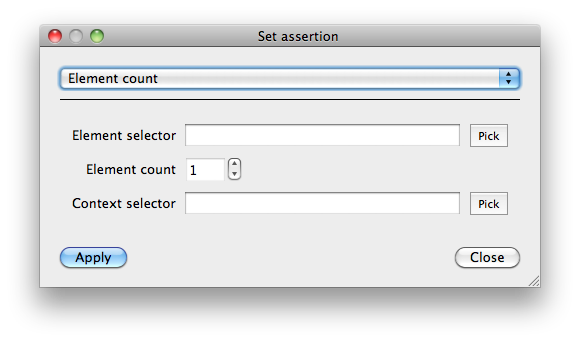
\includegraphics[width=\textwidth]{images/wp_tour/9_count_dialog.png}
\caption{Finestra per creare una nuova asserzione}
\label{fig:assertCountDialog}
\end{center}
\end{figure}

\section{Descrizione del primo esperimento}

La seconda fase dell'esperimento ha permesso di verificare il grado di flessibilità raggiunto dai test definiti attraverso lo strumento realizzato. Per fare ciò si è rieseguito il test su una versione successiva della piattaforma Wordpress. Per questa seconda prova è stata usata la versione 3.1.3, che durante la fase di progetto risultava essere la più recente, poiché essa presenta alcune modifiche nel layout del pannello di amministrazione rispetto alle versioni 2.X, mentre le funzionalità rimangono pressoché inalterate.

Una volta definito il test attraverso i passi appena descritti, esso è stato esportato in formato XML. Dopodiché si è modificato l'indirizzo di partenza, affinché puntasse alla nuova versione di Wordpress installata in locale.

Affinché lo stesso test venisse eseguito senza errori su entrambe le versioni, è stato necessario modificare solamente due dei selettori generati automaticamente dallo strumento.

Nello specifico, il valore dell'attributo id del campo di testo per inserire una nuova categoria nella pagina di modifica di un articolo è stato modificato da \verb|#newcat| a \verb|#newcategory|. Poiché la modifica è avvenuta sull'attributo id, il selettore generato dallo strumento non è stato in grado di selezionare il nodo del DOM nella versione più recente della piattaforma.

Allo stesso modo, poiché nella versione più recente è stato corretto un errore di battitura per l'attributo id assegnato al pulsante per aggiungere una nuova categoria, che è passato dal valore \verb|category-add-sumbit| al valore \verb|category-add-submit|, è stato necessario adattare il selettore ottenuto registrando il test.

Durante queste prove è stata inoltre dimostrata in vari casi l'utilità pratica dell'algoritmo che si occupa di fornire selettori alternativi a quelli definiti in fase di acquisizione del test, nel caso in cui non sia possibile reperire l'elemento al primo tentativo.

Uno dei casi interessanti ha riguardato l'elenco principale degli articoli salvati nel database. Le righe della tabella generate in maniera dinamica possiedono un attributo id, che ha come suffisso la chiave primaria del record nel database corrispondente a ciascun articolo, come è possibile osservare in figura ~\ref{fig:trId}. Se il selettore generato per individuare il link contenuto all'interno della prima cella di ogni riga contenesse l'attributo id assegnato al tag \verb|tr|, i risultati dei test sarebbero condizionati dal valore della chiave primaria di ogni record nel database e l'azione definita potrebbe fallire o avere successo a seconda di questo fattore, che dovrebbe essere invece un dettaglio implementativo non influente ai fini delle verifiche effettuate.

\begin{figure}[htbp]
\begin{center}
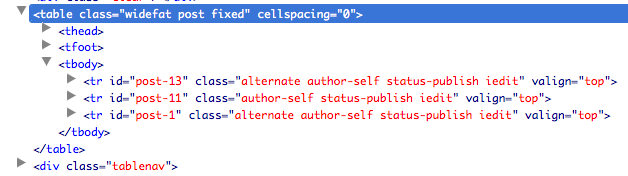
\includegraphics[width=\textwidth]{images/wp_tour/10_firebug_tr_id.png}
\caption{Attributi id per le righe della tabella contenente gli articoli salvati}
\label{fig:trId}
\end{center}
\end{figure}

L'algoritmo di generazione dei selettori riconosce questo schema tramite un'espressione regolare, siccome è tipico di molte applicazioni in cui il contenuto viene generato dinamicamente, ed ignora l'attributo id, riferendosi poi a quello successivo trovato risalendo nella gerarchia dell'albero DOM. Si confrontino come esempio i due selettori generati senza questo accorgimento per identificare il link alla pagina di modifica di un articolo, in base al frammento di codice HTML mostrato in figura ~\ref{fig:trId}:

Selettore generato senza modifiche:  \verb|#post-62 a:icontains(post+title)| 
\newline
Selettore generato tenendo conto dell'attributi id generato dinamicamente:  \verb|#the-list a:icontains(post+title)| 

Pertanto, è stato possibile eseguire lo stesso test sulle due versioni nonostante esse utilizzino due database separati, con valori differenti per le chiavi primarie dei record.